% Practice questions retained from Chapter 3, with corrected interpretation prompts.

\clearpage
\section*{Practice A: Center}
\begin{enumerate}[label=A\arabic*.,leftmargin=2.5em,itemsep=10pt]
  \item Find the mean, median, and mode of each data set.
    \begin{enumerate}[label=(\alph*), itemsep=5pt]
      \item $4,\; 7,\; 7,\; 9,\; 11,\; 13,\; 7,\; 6$
      \item $22,\; 18,\; 30,\; 22,\; 25,\; 18,\; 29,\;
             22,\; 31$
      \item $0.5,\; 1.2,\; 0.8,\; 1.5,\; 0.9,\; 1.1$
    \end{enumerate}

  \item The following data records the number of customer
    complaints received by a store over ten days:
    \[ 3,\; 0,\; 5,\; 2,\; 1,\; 4,\; 2,\; 8,\; 2,\; 3. \]
    \begin{enumerate}[label=(\alph*), itemsep=4pt]
      \item Find the mean, median, and mode.
      \item On day 8, a particularly difficult situation led
        to 8 complaints. Describe the effect of removing this
        value from the data set on each of the three measures.
    \end{enumerate}

  \item A real estate agent reports that the mean home price
    in a neighborhood is \$420{,}000, but the median is
    \$285{,}000.
    In two complete sentences, explain what this difference
    tells a potential buyer about the distribution of home
    prices in the neighborhood.

  \item Seven students took a test. Six of them scored
    $72, 78, 84, 80, 76, 88$.
    The mean score for all seven students is $80$.
    What did the seventh student score?
    Show your work.

\end{enumerate}

\clearpage
\section*{Practice B: Range}
\begin{enumerate}[label=B\arabic*.,leftmargin=2.5em,itemsep=10pt]
  \item Find the range of each data set.
    \begin{enumerate}[label=(\alph*), itemsep=4pt]
      \item $14,\; 22,\; 9,\; 31,\; 18,\; 27$
      \item $-5,\; 0,\; 3,\; -2,\; 8,\; -7,\; 1$
      \item $0.4,\; 1.1,\; 0.7,\; 1.8,\; 0.3$
    \end{enumerate}

  \item Two delivery drivers recorded the following number
    of deliveries per day over five days.
    \begin{center}
    \renewcommand{\arraystretch}{1.4}
    \begin{tabular}{lrrrrr}
    \toprule
    & Day 1 & Day 2 & Day 3 & Day 4 & Day 5 \\
    \midrule
    Driver A & 12 & 14 & 11 & 13 & 15 \\
    Driver B & 8  & 18 & 10 & 16 & 13 \\
    \bottomrule
    \end{tabular}
    \end{center}
    \begin{enumerate}[label=(\alph*), itemsep=4pt]
      \item Compute the mean and range for each driver.
      \item Which driver is more consistent?
        Justify your answer using the range.
    \end{enumerate}

  \item A data set has a range of $40$ and a minimum value
    of $15$. What is the maximum value?

\end{enumerate}

\clearpage
\section*{Practice C: Sample standard deviation}
\begin{enumerate}[label=C\arabic*.,leftmargin=2.5em,itemsep=10pt]
  \item Compute the sample standard deviation of each data set.
    Show all steps using the deviation table.
    \begin{enumerate}[label=(\alph*), itemsep=6pt]
      \item $3,\; 5,\; 5,\; 7$
      \item $10,\; 20,\; 30,\; 40$
      \item $6,\; 6,\; 9,\; 9$
    \end{enumerate}

  \item Without computing, decide which data set has a
    larger sample standard deviation. Explain your reasoning.
    \begin{enumerate}[label=(\alph*), itemsep=4pt]
      \item Set A: $50, 51, 50, 49, 50$ \quad
        Set B: $30, 40, 50, 60, 70$
      \item Set C: $2, 2, 2, 2, 2$ \quad
        Set D: $1, 2, 3, 4, 5$
    \end{enumerate}

  \item A data set has five values with mean $\bar{x} = 10$.
    The squared deviations are $4, 1, 0, 1, 4$.
    Compute the sample standard deviation without knowing the
    original values.

  \item Two machines fill bottles with juice.
    Machine A fills to $250, 251, 249, 250, 250$ mL.
    Machine B fills to $245, 255, 248, 253, 249$ mL.
    \begin{enumerate}[label=(\alph*), itemsep=4pt]
      \item Compute the mean and sample standard deviation for
        each machine.
      \item Which machine is more consistent?
        Justify using the sample standard deviation.
    \end{enumerate}

\end{enumerate}

\clearpage
\section*{Practice D: Interpreting summaries}
\begin{enumerate}[label=D\arabic*.,leftmargin=2.5em,itemsep=10pt]
  \item For each data set, compute all five statistics:
    mean, median, mode, range, and sample standard deviation.
    Use the values and statistics to explain how an extreme value affects the summaries. Which center better describes a typical observation? Explain.
    \begin{enumerate}[label=(\alph*), itemsep=6pt]
      \item $12,\; 14,\; 14,\; 15,\; 16,\; 17,\; 14$
      \item $5,\; 6,\; 7,\; 8,\; 9,\; 10,\; 85$
    \end{enumerate}

  \item A meteorologist records daily rainfall (in inches)
    for two weeks:
    \[ 0,\; 0,\; 0.2,\; 0,\; 1.4,\; 0,\; 0,\;
       0.1,\; 0,\; 0,\; 2.1,\; 0,\; 0,\; 0. \]
    \begin{enumerate}[label=(\alph*), itemsep=4pt]
      \item Find the mean, median, and mode.
      \item Which measure of center best represents a
        typical day?
        Justify in two sentences.
    \end{enumerate}

  \item A dataset has mean $20$ and sample standard deviation $3$.
    Another has mean $20$ and sample standard deviation $10$.
    \begin{enumerate}[label=(\alph*), itemsep=4pt]
      \item Sketch a rough histogram for each,
        placing the center at $20$.
      \item What does a larger sample standard deviation indicate
        about the distribution of values?
    \end{enumerate}

\end{enumerate}

\clearpage
\section*{Practice E: Reading graphs}
\begin{enumerate}[label=E\arabic*.,leftmargin=2.5em,itemsep=10pt]
  \item The histogram below shows the distribution of
    heights (in inches) for a sample of 40 adults.

  \begin{center}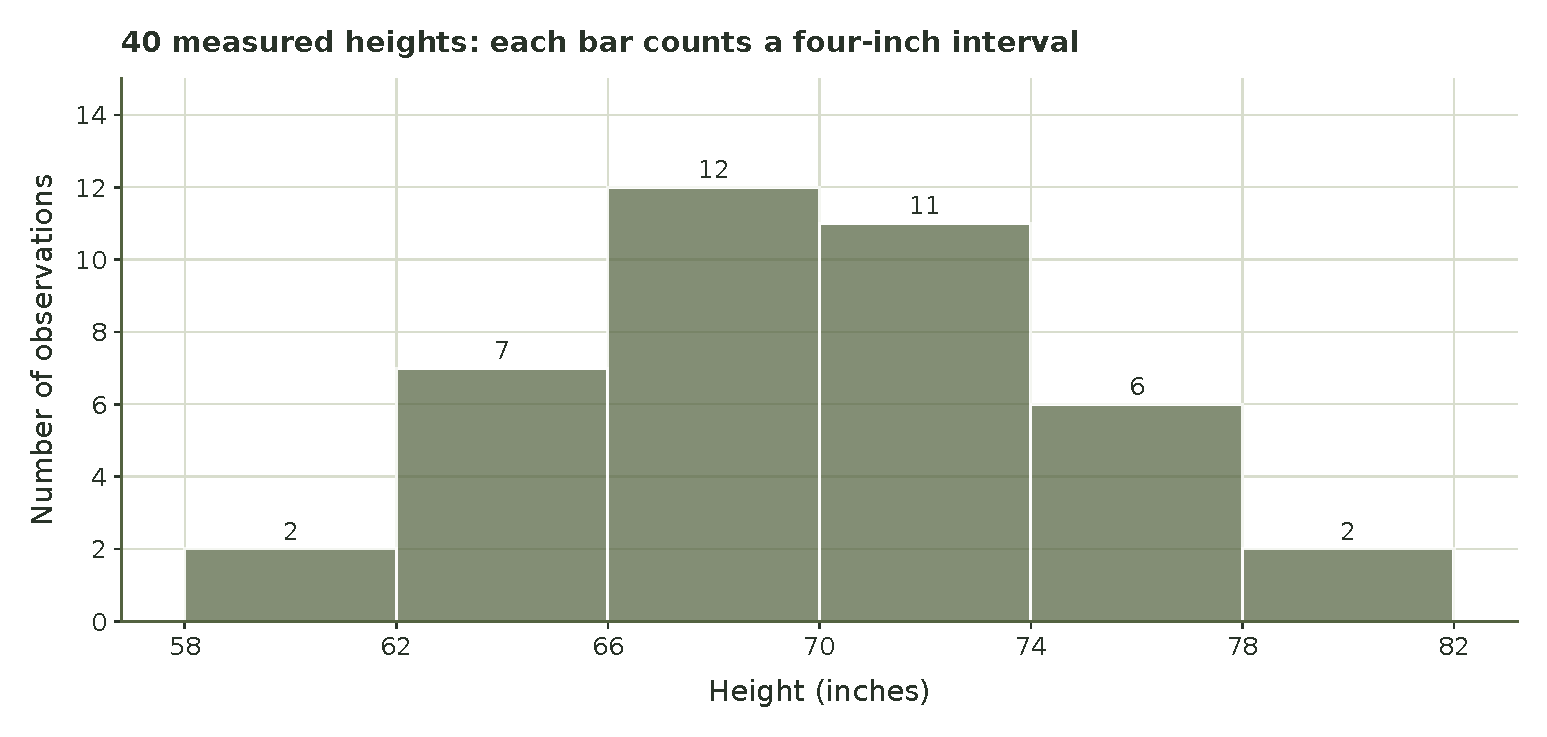
\includegraphics[width=\linewidth,height=2.8in,keepaspectratio]{../assets/week3/height-histogram.pdf}\end{center}

    \begin{enumerate}[label=(\alph*), itemsep=4pt]
      \item Which interval has the largest count? Is that a majority of the observations?
      \item Is the distribution symmetric or skewed?
      \item Would you expect the mean to be close to the
        median? Explain in one sentence.
    \end{enumerate}

  \item Sketch two histograms with the same center but
    different spreads. Label the center on both.
    Below each sketch, write one sentence describing
    what each distribution tells an observer about
    the data.

  \item A data set has mean $30$ and sample standard deviation $2$.
    A second data set has mean $30$ and sample standard deviation $8$.
    An observation of $36$ is taken.
    \begin{enumerate}[label=(\alph*), itemsep=4pt]
      \item How many sample standard deviations above the mean
        is $36$ in each data set?
      \item In which data set is the value $36$ more
        unusual? Explain in one sentence.
    \end{enumerate}

\end{enumerate}

\clearpage
\section*{Practice F: Weighted averages}
\begin{enumerate}[label=F\arabic*.,leftmargin=2.5em,itemsep=10pt]
\item Scores 70 and 90 receive weights 0.25 and 0.75. Find the weighted result, compare it with the ordinary mean, and check that it lies between the two values.
\item Values 2, 5, 8, 10 receive weights 0.10, 0.20, 0.60, 0.10. Check the weight total, calculate every contribution, and find the weighted result. What does the largest weight tell you?
\item In a whole-sentence illustration, positions 2, 3, 5, 6, 8 receive weights 0.10, 0.05, 0.70, 0.05, 0.10. Find the weighted position. Explain why a decimal result does not designate a fractional word. Why would a next-token generator need to exclude words that are not available yet?
\end{enumerate}
\section*{Practice G: Changing every value}
\begin{enumerate}[label=G\arabic*.,leftmargin=2.5em,itemsep=10pt]
\item A sample has mean 20 and sample SD 3. Separately, (a) add 5 to every value and (b) multiply every original value by 2. Give the resulting mean and SD for each change, and explain through distances from the mean.
\end{enumerate}

\clearpage
\section*{Chapter 3 Review}
\begin{enumerate}[label=R\arabic*.,leftmargin=2.5em,itemsep=10pt]

  \item The following data records the number of hours per
    week a sample of 10 students spend on homework:
    \[ 4,\; 7,\; 5,\; 8,\; 6,\; 5,\; 9,\; 4,\; 6,\; 6. \]
    \begin{enumerate}[label=(\alph*), itemsep=4pt]
      \item Find the mean, median, mode, and range.
      \item Construct the deviation table and compute
        the sample standard deviation.
      \item Describe the center and spread of this data
        set in two complete sentences.
    \end{enumerate}

  \item A company tracks the number of sick days taken
    by employees in one year.
    The data for eight employees is:
    \[ 0,\; 1,\; 2,\; 1,\; 0,\; 3,\; 1,\; 18. \]
    \begin{enumerate}[label=(\alph*), itemsep=4pt]
      \item Compute the mean and median.
      \item Which measure better represents a typical
        employee? Explain.
      \item If the value $18$ is removed, how do the mean
        and median each change? Compute both.
    \end{enumerate}

  \item Two students each score a mean of $80$ on five
    exams. Student A's scores are
    $78, 79, 80, 81, 82$.
    Student B's scores are
    $60, 70, 80, 90, 100$.
    Without computing, predict which student has the
    larger sample standard deviation.
    Then compute both sample standard deviations to verify.

  \item A data set has six values.
    Five of them are $12, 15, 14, 13, 16$.
    The mean of all six values is $14$.
    Find the sixth value.

  \item A histogram of test scores is skewed left.
    \begin{enumerate}[label=(\alph*), itemsep=4pt]
      \item What does it mean for a histogram to be
        skewed left?
      \item Would you expect the mean to be greater than,
        equal to, or less than the median?
        Explain in two sentences.
    \end{enumerate}

  \item The temperatures recorded over five days in two
    cities are:
    \begin{center}
    \renewcommand{\arraystretch}{1.4}
    \begin{tabular}{lrrrrr}
    \toprule
    & Day 1 & Day 2 & Day 3 & Day 4 & Day 5 \\
    \midrule
    City A & 68 & 70 & 69 & 71 & 67 \\
    City B & 55 & 62 & 74 & 79 & 85 \\
    \bottomrule
    \end{tabular}
    \end{center}
    \begin{enumerate}[label=(\alph*), itemsep=4pt]
      \item Compute the mean for each city.
      \item Compute the range and sample standard deviation
        for each city.
      \item Which city has more consistent temperatures?
        Justify using both spread measures.
    \end{enumerate}

  \item A quality control engineer samples 6 ball bearings
    and measures their diameters (in mm):
    \[ 9.98,\; 10.01,\; 10.00,\; 9.99,\; 10.02,\; 10.00. \]
    \begin{enumerate}[label=(\alph*), itemsep=4pt]
      \item Compute the mean and sample standard deviation.
      \item The specification requires that all bearings
        fall within $0.03$ mm of the target diameter of
        $10.00$ mm. Do all sampled bearings meet this
        requirement?
    \end{enumerate}

\end{enumerate}
